\documentclass[12pt,a4paper]{article}

\usepackage[margin=1in]{geometry}
\usepackage{amsmath, amssymb, amsthm}
\usepackage{mathtools}
\usepackage{enumitem}
\usepackage{booktabs}
\usepackage{array}
\usepackage{xcolor}
\usepackage{tikz}
\usetikzlibrary{arrows.meta, positioning}

\setlength{\parindent}{0pt}
\setlength{\parskip}{6pt}

\newtheoremstyle{lecturestyle}
  {8pt}
  {8pt}
  {\normalfont}
  {}
  {\bfseries}
  {.}
  {0.5em}
  {}

\theoremstyle{lecturestyle}
\newtheorem{definition}{Definition}
\newtheorem{example}{Example}
\newtheorem{remark}{Remark}

\newenvironment{answer}
{\par\textbf{Answer.}\ }
{\hfill$\square$\par}

\newcommand{\Prob}{\mathbb{P}}
\newcommand{\E}{\mathbb{E}}

\title{\textbf{Lecture 7: Introduction to Markov Chains}}
\author{MA4034: Time Series and Stochastic Processes}
\date{}

\begin{document}
\maketitle

\section{Motivation: Playing Roulette}

Suppose we play a simplified roulette game. In American roulette there are 38 slots. If the ball lands on an odd numbered slot, the player wins \$1. If the ball lands on an even numbered slot or one of the two special slots, the player loses \$1.

\[
\Prob(\text{win})=\frac{18}{38}, \qquad
\Prob(\text{lose})=\frac{20}{38}.
\]

Therefore the losing probability is larger than the winning probability. This is common in gambling games: the rules are designed so that, in the long run, the player is more likely to lose than to win.

Assume that the player starts with \$10. Let
\[
X_n=\text{amount of money the player has after } n \text{ games}.
\]
Then
\[
X_0=10.
\]
At each game,
\[
X_{n+1}=
\begin{cases}
X_n+1, & \text{with probability } \frac{18}{38},\\
X_n-1, & \text{with probability } \frac{20}{38}.
\end{cases}
\]

For example, after one game the player may have \$11 or \$9. After two games the player may have \$12, \$10, or \$8. The value \$10 can be reached in different ways:
\[
10 \rightarrow 11 \rightarrow 10,
\qquad
10 \rightarrow 9 \rightarrow 10.
\]
Thus there may be many paths leading to the same state.

\begin{center}
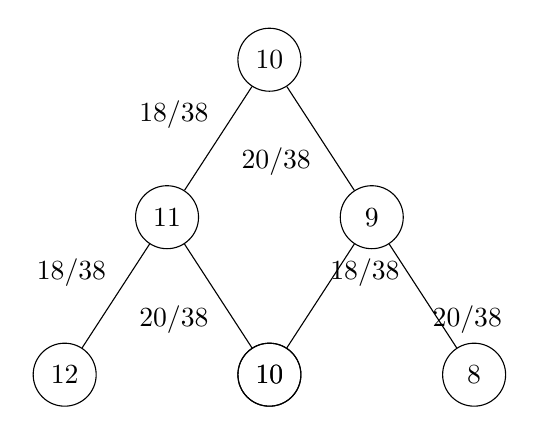
\begin{tikzpicture}[
  state/.style={circle, draw, minimum size=8mm},
  edge/.style={-{Latex[length=2mm]}, thick},
  level distance=20mm,
  sibling distance=26mm
]
\node[state] (x0) {$10$}
  child {node[state] (x1a) {$11$}
    child {node[state] {$12$} edge from parent node[above left] {$18/38$}}
    child {node[state] {$10$} edge from parent node[below left] {$20/38$}}
    edge from parent node[above left] {$18/38$}
  }
  child {node[state] (x1b) {$9$}
    child {node[state] {$10$} edge from parent node[above right] {$18/38$}}
    child {node[state] {$8$} edge from parent node[below right] {$20/38$}}
    edge from parent node[below left] {$20/38$}
  };
\end{tikzpicture}
\end{center}

\textbf{Analogy.} Think of the player's money as their position on a staircase. Each roulette spin moves them one step up with probability $18/38$ or one step down with probability $20/38$. To know the possible next step, we only need to know the current stair, not exactly how the player reached it.

\section{The Markov Property}

Many stochastic processes have some dependence on the past. In a Markov chain, the dependence is usually only on the most recent value. This is called lag-one dependence.

\begin{definition}[Markov Property]
Let $\{X_0,X_1,X_2,\ldots\}$ be a sequence of discrete random variables taking values in a state space $S$. The process is called a \textbf{Markov chain} if
\[
\Prob(X_{n+1}=j \mid X_0=i_0,\ldots,X_{n-1}=i_{n-1},X_n=i)
=
\Prob(X_{n+1}=j \mid X_n=i)
\]
for all states $i_0,\ldots,i_{n-1},i,j\in S$ and all $n\geq 0$.
\end{definition}

This means that, given the present state, the future does not depend on the earlier past.

\[
\text{Future} \quad \perp \quad \text{Past} \mid \text{Present}.
\]

In simple words:
\[
\text{Next state depends on the current state, not on the full history.}
\]

\begin{remark}
The Markov property does not say that the past is useless in every sense. It says that once the current state is known, earlier states give no extra information about the next state.
\end{remark}

\textbf{Analogy.} Suppose you are using a GPS. If the GPS knows your current location, it can suggest the next road. It does not need to know every road you used earlier to arrive there. Similarly, a Markov chain uses the current state as the relevant summary of the past.

\subsection{First-Order and Higher-Order Markov Chains}

A first-order Markov chain depends only on the immediately previous value:
\[
\Prob(X_{n+1}=j \mid X_n=i).
\]

A second-order Markov chain may depend on the previous two values:
\[
\Prob(X_{n+1}=j \mid X_n=i, X_{n-1}=k).
\]

However, many higher-order Markov chains can be rewritten as first-order Markov chains by increasing the state description. For example, instead of using $X_n$ as the state, we can use the pair
\[
Y_n=(X_{n-1},X_n).
\]
Then $\{Y_n\}$ can be treated as a first-order Markov chain.

\section{Time-Homogeneous Markov Chains}

\begin{definition}[Time-Homogeneous Markov Chain]
A Markov chain is called \textbf{time-homogeneous} if the transition probabilities do not change with time. That is,
\[
\Prob(X_{n+1}=j\mid X_n=i)
\]
is the same for all values of $n$.
\end{definition}

For a time-homogeneous chain, the probability of moving from state $i$ to state $j$ in one step is denoted by
\[
p_{ij}=\Prob(X_{n+1}=j\mid X_n=i), \qquad i,j\in S.
\]

Here $p_{ij}$ means:
\[
\text{probability of moving from state } i \text{ to state } j \text{ in one step.}
\]

For example, in the roulette problem,
\[
p_{i,i+1}=\frac{18}{38}, \qquad p_{i,i-1}=\frac{20}{38}
\]
for all positive states $i\geq 1$. If the player reaches \$0, the player is ruined and cannot continue, so
\[
p_{00}=1.
\]

\textbf{Analogy.} Time-homogeneous means the rules of the game do not change. If winning today moves the player from \$10 to \$11 with probability $18/38$, then the same kind of move tomorrow also has probability $18/38$.

\section{Transition Probabilities}

The numbers $p_{ij}$ are called \textbf{transition probabilities}. They describe how the chain moves from one state to another.

The transition probabilities must satisfy two conditions:
\[
p_{ij}\geq 0 \qquad \text{for all } i,j\in S,
\]
and
\[
\sum_{j\in S}p_{ij}=1 \qquad \text{for every fixed } i\in S.
\]

The second condition says that if the chain is currently in state $i$, then it must move to one of the possible next states. Therefore the probabilities of all possible next states must add to 1.

\begin{example}[Roulette Transition Probabilities]
In the roulette game, if the player currently has \$10, then the next amount can be \$11 or \$9:
\[
p_{10,11}=\frac{18}{38}, \qquad p_{10,9}=\frac{20}{38}.
\]
The row sum is
\[
p_{10,11}+p_{10,9}
=\frac{18}{38}+\frac{20}{38}
=1.
\]
\end{example}

\section{State Space}

\begin{definition}[State Space]
The \textbf{state space} $S$ is the set of all possible values that the process can take.
\end{definition}

In the roulette example, if the player can continue indefinitely and cannot go below \$0, the state space is
\[
S=\{0,1,2,3,\ldots\}.
\]
This is an infinite state space.

The state $0$ is special. Once the player reaches \$0, the player is ruined and cannot play anymore. Therefore
\[
\Prob(X_{n+1}=0\mid X_n=0)=1.
\]
Such a state is called an absorbing state.

\begin{definition}[Absorbing State]
A state $i$ is called an \textbf{absorbing state} if, once the chain enters state $i$, it stays there forever. Mathematically,
\[
p_{ii}=1.
\]
\end{definition}

\section{Transition Diagrams}

Instead of drawing a large tree diagram, we can represent a Markov chain using a \textbf{transition diagram}. A transition diagram is like a state diagram in Theory of Computing. The nodes are states, and the arrows show possible transitions.

For the roulette example:

\begin{center}
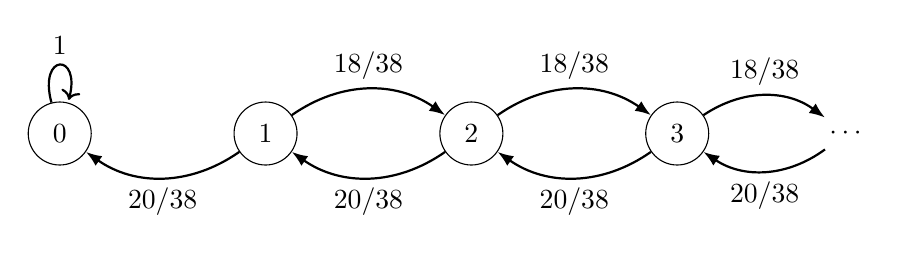
\begin{tikzpicture}[
  state/.style={circle, draw, minimum size=8mm},
  edge/.style={-{Latex[length=2mm]}, thick},
  bend angle=35
]
\node[state] (0) {$0$};
\node[state, right=18mm of 0] (1) {$1$};
\node[state, right=18mm of 1] (2) {$2$};
\node[state, right=18mm of 2] (3) {$3$};
\node[right=14mm of 3] (dots) {$\cdots$};

\draw[edge] (0) edge[loop above] node {$1$} (0);
\draw[edge] (1) edge[bend left] node[above] {$18/38$} (2);
\draw[edge] (2) edge[bend left] node[below] {$20/38$} (1);
\draw[edge] (2) edge[bend left] node[above] {$18/38$} (3);
\draw[edge] (3) edge[bend left] node[below] {$20/38$} (2);
\draw[edge] (1) edge[bend left] node[below] {$20/38$} (0);
\draw[edge] (3) edge[bend left] node[above] {$18/38$} (dots);
\draw[edge] (dots) edge[bend left] node[below] {$20/38$} (3);
\end{tikzpicture}
\end{center}

The states represent the amount of money the player has.

\section{Finite-State Example: Genetics}

Consider a gene in a plant with two alleles, $A$ and $a$. The possible genotypes are
\[
AA,\quad Aa,\quad aa.
\]
Suppose the plant is crossed with a plant of the same genotype repeatedly. The genotype of the offspring can be modeled as a Markov chain because the offspring genotype depends only on the parent genotype, not on the grandparent genotype.

The state space is
\[
S=\{AA,Aa,aa\}.
\]

The transition diagram is:

\begin{center}
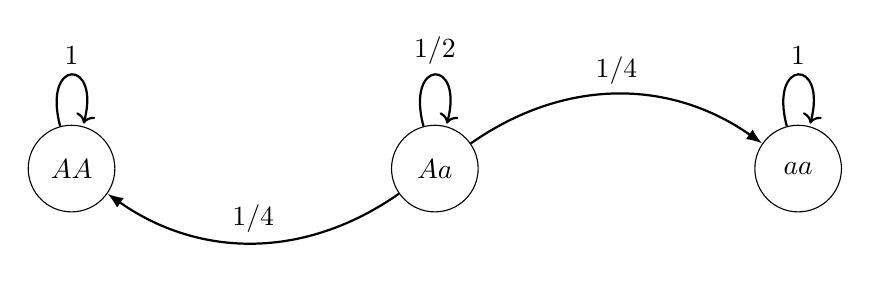
\begin{tikzpicture}[
  state/.style={circle, draw, minimum size=11mm},
  edge/.style={-{Latex[length=2mm]}, thick},
  bend angle=35
]
\node[state] (AA) {$AA$};
\node[state, right=35mm of AA] (Aa) {$Aa$};
\node[state, right=35mm of Aa] (aa) {$aa$};

\draw[edge] (AA) edge[loop above] node {$1$} (AA);
\draw[edge] (aa) edge[loop above] node {$1$} (aa);
\draw[edge] (Aa) edge[loop above] node {$1/2$} (Aa);
\draw[edge] (Aa) edge[bend left] node[above] {$1/4$} (AA);
\draw[edge] (Aa) edge[bend left] node[above] {$1/4$} (aa);
\end{tikzpicture}
\end{center}

From state $Aa$, the offspring possibilities are:
\[
AA,\quad Aa,\quad aA,\quad aa.
\]
Since $Aa$ and $aA$ represent the same genotype, the probabilities are:
\[
\Prob(AA)=\frac14,\qquad
\Prob(Aa)=\frac12,\qquad
\Prob(aa)=\frac14.
\]

\section{Transition Matrix}

When the state space is finite, it is convenient to summarize the transition probabilities in a matrix.

\begin{definition}[Transition Matrix]
For a finite-state Markov chain with states $S=\{1,2,\ldots,m\}$, the \textbf{transition matrix} is
\[
P=(p_{ij}),
\]
where the entry in row $i$ and column $j$ is
\[
p_{ij}=\Prob(X_{n+1}=j\mid X_n=i).
\]
\end{definition}

Rows represent the current state, and columns represent the next state. Therefore each row is a probability distribution over the possible next states.

For the genetics example, using the order
\[
S=\{AA,Aa,aa\},
\]
the transition matrix is
\[
P=
\begin{pmatrix}
1 & 0 & 0\\
\frac14 & \frac12 & \frac14\\
0 & 0 & 1
\end{pmatrix}.
\]

Notice that every row adds to 1:
\[
1+0+0=1,
\]
\[
\frac14+\frac12+\frac14=1,
\]
\[
0+0+1=1.
\]

\begin{remark}
A transition matrix is always a square matrix because the rows and columns both correspond to the same state space.
\end{remark}

\subsection{Infinite Transition Matrix}

For the roulette example, the state space is infinite:
\[
S=\{0,1,2,3,\ldots\}.
\]
The transition matrix is therefore an infinite square matrix:
\[
P=
\begin{pmatrix}
1 & 0 & 0 & 0 & 0 & \cdots\\
\frac{20}{38} & 0 & \frac{18}{38} & 0 & 0 & \cdots\\
0 & \frac{20}{38} & 0 & \frac{18}{38} & 0 & \cdots\\
0 & 0 & \frac{20}{38} & 0 & \frac{18}{38} & \cdots\\
\vdots & \vdots & \vdots & \vdots & \vdots & \ddots
\end{pmatrix}.
\]

The first row shows that state 0 is absorbing:
\[
p_{00}=1.
\]

\section{Time Dynamics of a Markov Chain}

The transition matrix describes one-step movement. Often, we want to know what happens after two or more steps.

The two-step transition probability is
\[
p_{ij}^{(2)}=\Prob(X_2=j\mid X_0=i).
\]

To move from state $i$ to state $j$ in two steps, the chain must pass through some intermediate state $k$. Using the law of total probability,
\[
p_{ij}^{(2)}
=\sum_{k\in S}\Prob(X_2=j,X_1=k\mid X_0=i).
\]
Then,
\[
p_{ij}^{(2)}
=\sum_{k\in S}\Prob(X_2=j\mid X_1=k,X_0=i)\Prob(X_1=k\mid X_0=i).
\]
By the Markov property,
\[
\Prob(X_2=j\mid X_1=k,X_0=i)=\Prob(X_2=j\mid X_1=k)=p_{kj}.
\]
Also,
\[
\Prob(X_1=k\mid X_0=i)=p_{ik}.
\]
Therefore,
\[
p_{ij}^{(2)}=\sum_{k\in S}p_{ik}p_{kj}.
\]

This is exactly the $(i,j)$ entry of the matrix product $P^2$. Hence,
\[
P^{(2)}=P^2.
\]

More generally, the $n$-step transition matrix is
\[
P^{(n)}=P^n.
\]

\textbf{Analogy.} A one-step transition matrix is like a map showing where you can go in one move. Squaring the matrix gives all possible two-move routes, adding together the probabilities of every route that starts at $i$ and ends at $j$.

\section{Worked Examples}

\begin{example}[Checking Whether a Matrix is a Transition Matrix]
Consider
\[
P=
\begin{pmatrix}
0.2 & 0.8\\
0.6 & 0.4
\end{pmatrix}.
\]
Is $P$ a valid transition matrix?
\end{example}

\begin{answer}
To be a valid transition matrix, all entries must be non-negative and each row must sum to 1.

All entries are non-negative:
\[
0.2,0.8,0.6,0.4\geq 0.
\]
Row 1:
\[
0.2+0.8=1.
\]
Row 2:
\[
0.6+0.4=1.
\]
Therefore $P$ is a valid transition matrix.
\end{answer}

\begin{example}[One-Step Probabilities in the Roulette Chain]
In the roulette chain, suppose the player currently has \$5. Find
\[
\Prob(X_{n+1}=6\mid X_n=5)
\]
and
\[
\Prob(X_{n+1}=4\mid X_n=5).
\]
\end{example}

\begin{answer}
The player wins \$1 with probability $18/38$ and loses \$1 with probability $20/38$.

Therefore,
\[
\Prob(X_{n+1}=6\mid X_n=5)=\frac{18}{38}.
\]
Also,
\[
\Prob(X_{n+1}=4\mid X_n=5)=\frac{20}{38}.
\]
\end{answer}

\begin{example}[Two-Step Probability in the Genetics Chain]
For the genetics chain,
\[
P=
\begin{pmatrix}
1 & 0 & 0\\
\frac14 & \frac12 & \frac14\\
0 & 0 & 1
\end{pmatrix},
\]
using the order $S=\{AA,Aa,aa\}$, find
\[
\Prob(X_2=AA\mid X_0=Aa).
\]
\end{example}

\begin{answer}
We need the two-step transition probability from $Aa$ to $AA$. This is the entry in row $Aa$ and column $AA$ of $P^2$.

Using
\[
p_{ij}^{(2)}=\sum_{k\in S}p_{ik}p_{kj},
\]
we get
\[
p_{Aa,AA}^{(2)}
=p_{Aa,AA}p_{AA,AA}
+p_{Aa,Aa}p_{Aa,AA}
+p_{Aa,aa}p_{aa,AA}.
\]
Substitute the values:
\[
p_{Aa,AA}^{(2)}
=\left(\frac14\right)(1)
+\left(\frac12\right)\left(\frac14\right)
+\left(\frac14\right)(0).
\]
Therefore,
\[
p_{Aa,AA}^{(2)}
=\frac14+\frac18+0
=\frac38.
\]
Thus,
\[
\Prob(X_2=AA\mid X_0=Aa)=\frac38.
\]
\end{answer}

\begin{example}[Converting a Second-Order Chain to a First-Order Chain]
Suppose a process satisfies
\[
\Prob(X_{n+1}\mid X_n,X_{n-1},X_{n-2},\ldots)
=\Prob(X_{n+1}\mid X_n,X_{n-1}).
\]
Explain how it can be represented as a first-order Markov chain.
\end{example}

\begin{answer}
The process is second-order because the next value depends on the previous two values. Define a new process
\[
Y_n=(X_{n-1},X_n).
\]
Then the next value is
\[
Y_{n+1}=(X_n,X_{n+1}).
\]
To determine $Y_{n+1}$, we only need $Y_n=(X_{n-1},X_n)$ because the distribution of $X_{n+1}$ depends only on $X_n$ and $X_{n-1}$.

Therefore $\{Y_n\}$ is a first-order Markov chain.
\end{answer}

\section{Summary}

\begin{itemize}[leftmargin=1.2cm]
    \item A stochastic process is a collection of random variables indexed by time.
    \item A Markov chain is a stochastic process where the next state depends only on the current state.
    \item The Markov property is
    \[
    \Prob(X_{n+1}=j\mid X_0,\ldots,X_n=i)=\Prob(X_{n+1}=j\mid X_n=i).
    \]
    \item A time-homogeneous Markov chain has transition probabilities that do not depend on time.
    \item The transition probability $p_{ij}$ is the probability of moving from state $i$ to state $j$ in one step.
    \item The transition probabilities must be non-negative and each row must sum to 1.
    \item A transition diagram represents states as nodes and transitions as arrows.
    \item A transition matrix stores all transition probabilities.
    \item For finite state spaces, the transition matrix is finite and square.
    \item For infinite state spaces, the transition matrix may be infinite but still square.
    \item Multi-step transition probabilities are found using powers of the transition matrix:
    \[
    P^{(n)}=P^n.
    \]
\end{itemize}

\section{Essay-Type Questions}

\begin{enumerate}[label=\textbf{Q\arabic*.}, leftmargin=1.2cm]
    \item Explain the Markov property. Why is it often described as ``the future depends on the present, not the past''?
    \item A roulette player starts with \$10 and wins \$1 with probability $18/38$ and loses \$1 with probability $20/38$. Model this as a Markov chain. Clearly state the state space, transition probabilities, and transition diagram.
    \item Define a time-homogeneous Markov chain. Explain the meaning of $p_{ij}$ and state the two conditions that transition probabilities must satisfy.
    \item Explain how a transition matrix represents a Markov chain. Use the genetics example with states $AA,Aa,aa$ to construct the transition matrix.
    \item Derive the formula for the two-step transition probability
    \[
    p_{ij}^{(2)}=\sum_{k\in S}p_{ik}p_{kj}.
    \]
    Explain why this is related to matrix multiplication.
    \item Explain how a second-order Markov chain can be converted into a first-order Markov chain.
\end{enumerate}

\section{Answers to Essay-Type Questions}

\subsection*{Answer 1}

The Markov property states that the conditional distribution of the next state depends only on the current state, not on the complete past history. Mathematically,
\[
\Prob(X_{n+1}=j\mid X_0=i_0,\ldots,X_{n-1}=i_{n-1},X_n=i)
=
\Prob(X_{n+1}=j\mid X_n=i).
\]

This means that, once we know the current state $X_n=i$, the earlier values $X_0,\ldots,X_{n-1}$ do not give extra information about the next state $X_{n+1}$.

It is described as ``the future depends on the present, not the past'' because the present state acts as a summary of all relevant past information.

For example, in the roulette game, if the player currently has \$10, the next amount will be \$11 with probability $18/38$ or \$9 with probability $20/38$. These probabilities do not depend on whether the player reached \$10 by first winning then losing, or first losing then winning.

\subsection*{Answer 2}

Let
\[
X_n=\text{amount of money the player has after }n\text{ games}.
\]
The player starts with
\[
X_0=10.
\]

The possible states are
\[
S=\{0,1,2,3,\ldots\}.
\]
State $0$ means the player has no money left and cannot continue. Therefore state $0$ is absorbing:
\[
p_{00}=1.
\]

For $i\geq 1$, the player can move to $i+1$ by winning or to $i-1$ by losing:
\[
p_{i,i+1}=\frac{18}{38},
\qquad
p_{i,i-1}=\frac{20}{38}.
\]
All other one-step transition probabilities are zero.

The transition diagram has states $0,1,2,3,\ldots$. There is a self-loop at state $0$ with probability $1$. From each positive state $i$, there is an arrow to $i+1$ with probability $18/38$ and an arrow to $i-1$ with probability $20/38$.

This is a Markov chain because the next amount of money depends only on the current amount, not on the full sequence of previous winnings and losses.

\subsection*{Answer 3}

A Markov chain is time-homogeneous if its transition probabilities do not change with time. That is,
\[
\Prob(X_{n+1}=j\mid X_n=i)
\]
is the same for all $n$.

For a time-homogeneous Markov chain, we write
\[
p_{ij}=\Prob(X_{n+1}=j\mid X_n=i).
\]
The symbol $p_{ij}$ means the probability of moving from state $i$ to state $j$ in one step.

The transition probabilities must satisfy:
\[
p_{ij}\geq 0 \qquad \text{for all }i,j\in S,
\]
and
\[
\sum_{j\in S}p_{ij}=1 \qquad \text{for every fixed }i\in S.
\]

The first condition says probabilities cannot be negative. The second condition says that, from any current state $i$, the chain must move to one of the possible next states, so the probabilities across the row must add to 1.

\subsection*{Answer 4}

A transition matrix is a square matrix that stores all one-step transition probabilities. The entry in row $i$ and column $j$ is
\[
p_{ij}=\Prob(X_{n+1}=j\mid X_n=i).
\]

Rows represent the current state, and columns represent the next state. Each row is a probability distribution, so every row must sum to 1.

In the genetics example, the possible genotypes are
\[
S=\{AA,Aa,aa\}.
\]
Using this order, we examine the transitions:

If the parent state is $AA$, the offspring state remains $AA$ with probability 1:
\[
(1,0,0).
\]
If the parent state is $Aa$, the offspring probabilities are
\[
\Prob(AA)=\frac14,\qquad
\Prob(Aa)=\frac12,\qquad
\Prob(aa)=\frac14.
\]
So the row is
\[
\left(\frac14,\frac12,\frac14\right).
\]
If the parent state is $aa$, the offspring state remains $aa$ with probability 1:
\[
(0,0,1).
\]

Therefore the transition matrix is
\[
P=
\begin{pmatrix}
1 & 0 & 0\\
\frac14 & \frac12 & \frac14\\
0 & 0 & 1
\end{pmatrix}.
\]

\subsection*{Answer 5}

The two-step transition probability is
\[
p_{ij}^{(2)}=\Prob(X_2=j\mid X_0=i).
\]
To go from state $i$ to state $j$ in two steps, the chain must pass through some intermediate state $k\in S$ at time 1.

Using the law of total probability,
\[
p_{ij}^{(2)}
=\sum_{k\in S}\Prob(X_2=j,X_1=k\mid X_0=i).
\]
Using the multiplication rule,
\[
p_{ij}^{(2)}
=\sum_{k\in S}\Prob(X_2=j\mid X_1=k,X_0=i)\Prob(X_1=k\mid X_0=i).
\]
By the Markov property,
\[
\Prob(X_2=j\mid X_1=k,X_0=i)=\Prob(X_2=j\mid X_1=k)=p_{kj}.
\]
Also,
\[
\Prob(X_1=k\mid X_0=i)=p_{ik}.
\]
Therefore,
\[
p_{ij}^{(2)}=\sum_{k\in S}p_{ik}p_{kj}.
\]

This is the same as matrix multiplication. The $(i,j)$ entry of $P^2$ is obtained by multiplying row $i$ of $P$ by column $j$ of $P$:
\[
(P^2)_{ij}=\sum_{k\in S}p_{ik}p_{kj}.
\]
Hence the two-step transition matrix is
\[
P^{(2)}=P^2.
\]

\subsection*{Answer 6}

A second-order Markov chain is a process where the next value depends on the previous two values:
\[
\Prob(X_{n+1}\mid X_n,X_{n-1},X_{n-2},\ldots)
=
\Prob(X_{n+1}\mid X_n,X_{n-1}).
\]

To convert it into a first-order Markov chain, define a new process whose state contains the last two values:
\[
Y_n=(X_{n-1},X_n).
\]
Then
\[
Y_{n+1}=(X_n,X_{n+1}).
\]

The distribution of $Y_{n+1}$ depends only on $Y_n$, because $Y_n$ already contains $X_{n-1}$ and $X_n$. Therefore,
\[
\Prob(Y_{n+1}\mid Y_n,Y_{n-1},\ldots)
=
\Prob(Y_{n+1}\mid Y_n).
\]

Thus the new process $\{Y_n\}$ is a first-order Markov chain. The important idea is that we enlarge the definition of a state so that the current state contains all information needed to predict the next state.

\end{document}
